%% This is emulateapj reformatting of the AASTEX sample document
%%
\documentclass{article}

\newcommand{\vdag}{(v)^\dagger}
\newcommand{\myemail}{james.casey-clyde@sjsu.edu}

\usepackage{amsmath,amsfonts}
%%\usepackage[numbers]{natbib}
\usepackage{graphicx}
\usepackage{caption}
\usepackage{subcaption}

%% You can insert a short comment on the title page using the command below.

%% If you wish, you may supply running head information, although
%% this information may be modified by the editorial offices.
%% The left head contains a list of authors,
%% usually a maximum of three (otherwise use et al.).  The right
%% head is a modified title of up to roughly 44 characters.
%% Running heads will not print in the manuscript style.

\title{Collapsed Cores in Globular Clusters}

%% This is the end of the preamble.  Indicate the beginning of the
%% paper itself with \begin{document}.

\begin{document}

%% LaTeX will automatically break titles if they run longer than
%% one line. However, you may use \\ to force a line break if
%% you desire.

\title{Machine Learning in Gravitational Wave Analysis}
\author{J. Andrew Casey-Clyde}
\maketitle


%% Notice that each of these authors has alternate affiliations, which
%% are identified by the \altaffilmark after each name.  Specify alternate
%% affiliation information with \altaffiltext, with one command per each
%% affiliation.


%% Mark off your abstract in the ``abstract'' environment. In the manuscript
%% style, abstract will output a Received/Accepted line after the
%% title and affiliation information. No date will appear since the author
%% does not have this information. The dates will be filled in by the
%% editorial office after submission.

\begin{abstract}
Gravitational wave detectors such as LIGO and Virgo offer new insights into our universe, yet also present challenges for analysis, primarily due to the sensitivity of the detectors to terrestrial sources of movement, as well as to the volume of data generated by these detectors. However, given the natures of these challenges, they are well suited to machine learning solutions. In this paper, I present techinques for the identification of transient events in LIGO timeseries data on all channels, as well as techniques for classifying these events as either terrestrial or non-terrestrial in origin. 
\end{abstract}

%% Keywords should appear after the \end{abstract} command. The uncommented
%% example has been keyed in ApJ style. See the instructions to authors
%% for the journal to which you are submitting your paper to determine
%% what keyword punctuation is appropriate.

%% Authors who wish to have the most important objects in their paper
%% linked in the electronic edition to a data center may do so in the
%% subject header.  Objects should be in the appropriate "individual"
%% headers (e.g. quasars: individual, stars: individual, etc.) with the
%% additional provision that the total number of headers, including each
%% individual object, not exceed six.  The \objectname{} macro, and its
%% alias \object{}, is used to mark each object.  The macro takes the object
%% name as its primary argument.  This name will appear in the paper
%% and serve as the link's anchor in the electronic edition if the name
%% is recognized by the data centers.  The macro also takes an optional
%% argument in parentheses in cases where the data center identification
%% differs from what is to be printed in the paper.

%%\keywords{globular clusters: general ---
%%globular clusters: individual(\objectname{NGC 6397},
%%\object{NGC 6624}, \objectname[M 15]{NGC 7078},
%%\object[Cl 1938-341]{Terzan 8})}

%% From the front matter, we move on to the body of the paper.
%% In the first two sections, notice the use of the natbib \citep
%% and \citet commands to identify citations.  The citations are
%% tied to the reference list via symbolic KEYs. The KEY corresponds
%% to the KEY in the \bibitem in the reference list below. We have
%% chosen the first three characters of the first author's name plus
%% the last two numeral of the year of publication as our KEY for
%% each reference.

\section{Introduction}
The search for gravitaional waves was a long one. Sparked in 1916 by Albert Einstein's theory of General Relativity, it wasn't until 100 years later, in 2016, that the first two gravitaitonal wave events were confirmed using data from Advanced LIGO's sensitive instruments \cite{TheLIGOScientificCollaboration2016} \cite{Abbott2016}. The sensitivity of LIGO instruments comes with the double edged sword of large quantities of data. Furthermore, this data is subject to large amounts of terrestrial noise, which can mimic transient gravitational wave events. This makes the data difficult for manual examination, making it a prime candidate for clustering and machine learning techniques.

In fact, multiple machine learning techniques have been explored specifically for the purposes of processing LIGO data, including both Artificial Neural Networks (ANN) \cite{Biswas2013} and Difference Boosting Neural Networks (DBNN) \cite{Mukund2016}. These techniques can be used, in conjunction with auxiliary channel data, to identify non-astrophysical transients, which may then be removed from the dataset. Once these datasets are removed, the remaining transients can then be further classified (such as by using hierarchical clustering algorithms) in order to determine potential transient categories, as well as how related those categories are morphologically.

\section{Methods}
In order to classify transients in the LIGO data, they must first be found. To this end, I apply the Kleine Welle algorithm, which decomposes wavelets into the time-scale domain and searches for regions of energy overdensities in the signal \cite{Biswas2013}\cite{Blackburn2007}. These techniques may be applied to all detector channels to extract transients, and in fact will be necessary for differentiating between terrestrial and astrophysical transient sources.

\subsection{Data Cleaning}
The LIGO gravitational wave data is characterized by Gaussian noise, with non-Gaussian transient events. As such, before applying the Kleine Welle algorithm to search for overdensities, it is useful to first whiten the data by taking it's Fourier transform and dividing by the amplitude spectral density (ASD), which is the square root of the power spectral density, and then transforming back \cite{LIGOScientificCollaboration}. This helps to suppress signal due to noise, enhancing transient signals. An example of the pre and post whitened ASD for the segment of data around GW150914 is shown in Figure \ref{fig:asd}.

\begin{figure}
\begin{subfigure}{\textwidth}
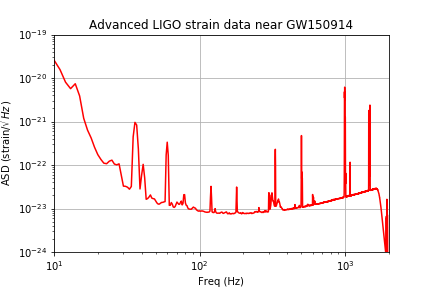
\includegraphics[width=\textwidth]{GW150914_prewhite.png}
\caption{ASD before whitening}
\label{fig:prewhite}
\end{subfigure}

\begin{subfigure}{\textwidth}
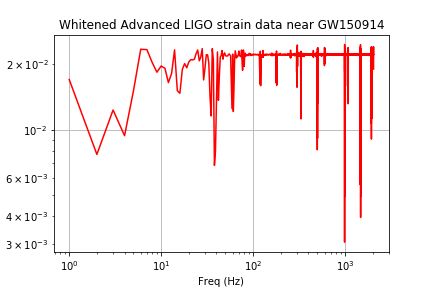
\includegraphics[width=\textwidth]{GW150914_white.png}
\caption{ASD after whitening}
\label{fig:postwhite}
\end{subfigure}
\caption{ASD vs. frequency for the Advanced LIGO data near GW150914, before and after whitening. Notice that in about the $80-300\mathrm{Hz}$ range, the noise is at a minumum, and relatively constant. This is the range we wish to search for transient events.}
\label{fig:asd}
\end{figure}

Additionally, a butterworth bandpass filter may be applied to the whitened data \cite{Blackburn2007}\cite{LIGOScientificCollaboration} in order to remove regions of large or fluctuating background noise, such as those regions outside $80-300\mathrm{Hz}$ in Figure \ref{fig:prewhite}.

\subsection{Event Identification}
Once the data has been whitened and bandpassed, it can be fed through the Kleine Welle algorithm. The algorithm works through the application of a dyadic wavelet decomposition, whose coefficients can be used to search for signal energy overdensities \cite{Biswas2013}\cite{Blackburn2007}. In general, the wavelet transform is defined by the equation \cite{Blackburn2007}\cite{Mallat1999}
\begin{equation}
W_{f}(u,s)=\int_{-\infty}^{+\infty}f(t)\frac{1}{\sqrt{s}}\psi^{*}\left(\frac{t-u}{s}\right)dt, \label{eq:wavtr}
\end{equation}
where $s$ is the scale. The calculation of this transformation can be made computationally inexpensive through the discretization of $s$ to a dyadic sequence, such that $s \in \{2^{j}\}_{j\in\mathbb{Z}}$ \cite{Blackburn2007}\cite{Mallat1999}.

Applying this to the LIGO timeseries data at multiple scales $j$ \cite{Wasilewski} yields a series of detail coefficients $D_{j}$ for each scale, with elements $d_{ij}$, whose values scale with signal energy and approach a zero mean Gaussian \cite{Blackburn2007}. We can threshold on these elements to look for outliers by using the standard deviation of each decomposition level, $\sigma_{j}$, such that $d_{ij}/4\sigma_{j} > 4$. Elements which pass this threshold are then normalized to create a set of square normalized coefficients such that
\begin{equation}
E_{j} = D_{j}^{2}/\sigma_{j}^{2} = \{\epsilon_{ij}\},
\end{equation}
where the elements $\epsilon_{ij}$ correspond to the same elements $d_{ij}$. Taking only those $\epsilon_{ij}$ whose corresponding detail coefficients passed the earlier thresholding, we can cluster these over time, decomposition scale, and normalized energy. The mean shift clustering method is particularly well suited to this problem, as it does not require prior knowledge or the number of clusters present \cite{Ivezic2014}, which in principle we cannot know for a given segment. An example of this clustering is shown in Figure \ref{fig:cluster}. The elements of a given cluster $C$ can then be added to form the total normalized cluster energy \cite{Blackburn2007},
\begin{equation}
E_{c} = \sum_{(i,j)\in C}\epsilon_{ij}. \label{eq:Ec}
\end{equation}
The significance of a cluster is then defined as \cite{Blackburn2007}
\begin{equation}
S=-\ln\int_{E_{c}}^{+\infty}\chi_{N}^{2}(E)dE, \label{eq:significance}
\end{equation}
where the number of degrees of freedom $N$ is the number of elements in the cluster. With this, it simply becomes a matter or thresholding the significance of each cluster.

\begin{figure}
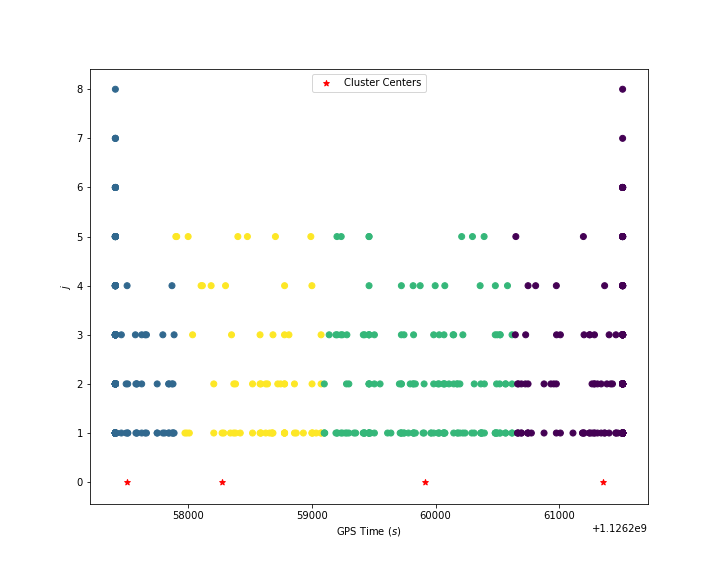
\includegraphics[width=\textwidth]{GW150914_cluster.png}
\caption{Square normalized coefficient clustering in the timeseries region around GW150914}
\label{fig:cluster}
\end{figure}

\subsection{Event Classification}
Once transients have been identified in the strain data, they can be classified using a neural network; in this case, I choose to use a Multi-Layered Perceptron (MLP), one of the more popular neural network models. For training data, we can use hardware injected events for astrophysical event classification. Additionally, we also need non-astrophysical events to train on. These can be generated by looking for events in each detector that do not overlap with events from the other detector (i.e., events in H1 that do not overlap with events from L1). By applying the hardware injections and independent events as labels, we can then form a set of data for training and testing.

\section{Analysis}
Keeping in mind that each LIGO science run contains data collected using progressively more sensitive instruments, I choose to apply these techniques to the first 2 weeks of the S6 data release \cite{LIGOScientificCollaboration2015}, from the most recent data collection run before Advanced LIGO instruments came online, which offers the best sensitivity for publically available data. Each data segment from each detector is then run through the Kleine Welle selection algorithm as described above. When a significant cluster is found, it is recorded in a data file, with start and end times, event length, the significance of the event, and the cluster center (in time, scale, and energy). Using this technique, I find 761 events from H1, and 912 events from L1.

To identify injection clusters, I compare the time coordinate of the cluster center to the the injection time periods, and find NUM Compact Binary Coalescence (CBC) injections, NUM Burst injections, and NUM Stochastic injections for H1, and NUM, NUM, and NUM CBC, Burst, and Stochastic injections, respectivley, for L1. As described above, I then split the data into training and testing, with the testing data achieving a score of SCORE.

\bibliography{library}
\bibliographystyle{unsrt}


\end{document}

%%
%% End of file `sample.tex'.
